\documentclass[a4paper,12pt]{article}


\usepackage{setspace}
\usepackage{xcolor}
\usepackage{graphicx}
\usepackage{geometry}
\usepackage{float}
\usepackage{titlesec}
\usepackage{subfigure}
\usepackage{caption}
\captionsetup{figurewithin=section}
\usepackage{amsmath}


\begin{document}

\title{\textbf{Homework 1}}
\author{Yunian Pan}
\maketitle{}

\section{Problem 1}

Select some typical values of d from \{1, \ldots, 40\}, the fitting lines are shown as below:

\begin{figure}[h]
\setcounter{subfigure}{0}
\centering
\subfigure[d=1]{
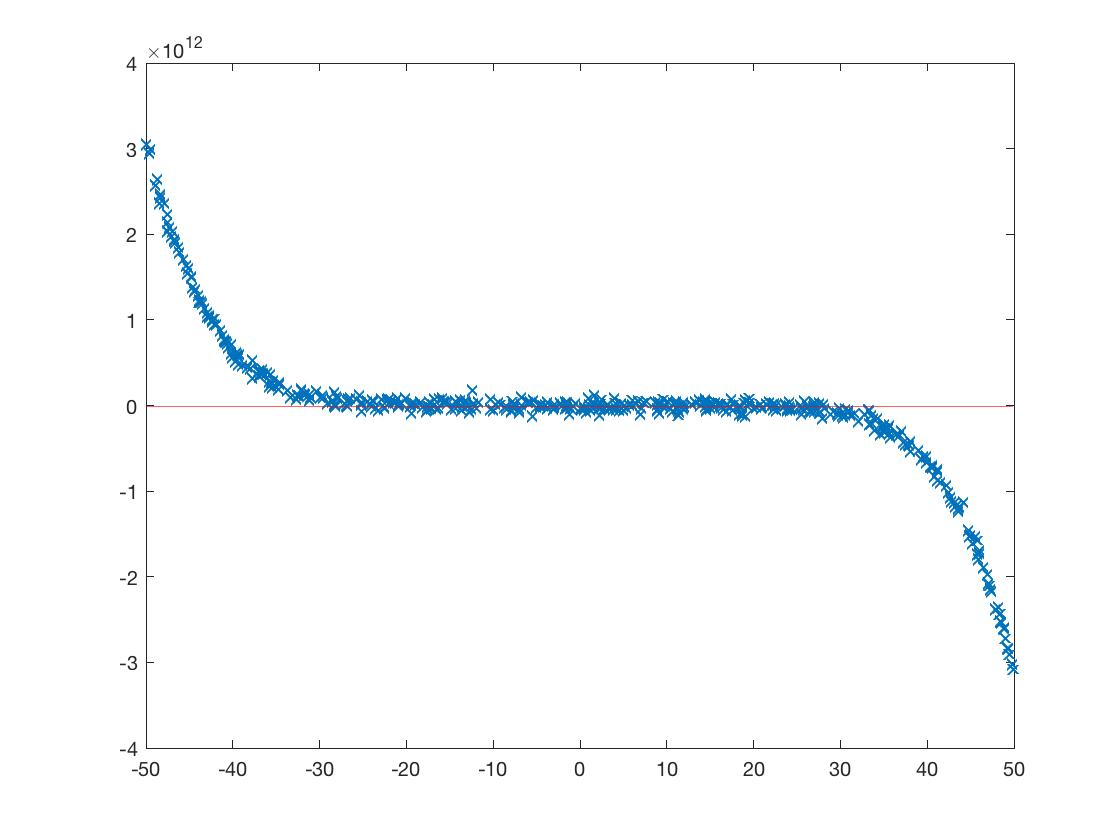
\includegraphics[width = .45\textwidth]{figure/d1.jpg}
}
\subfigure[d=2]{
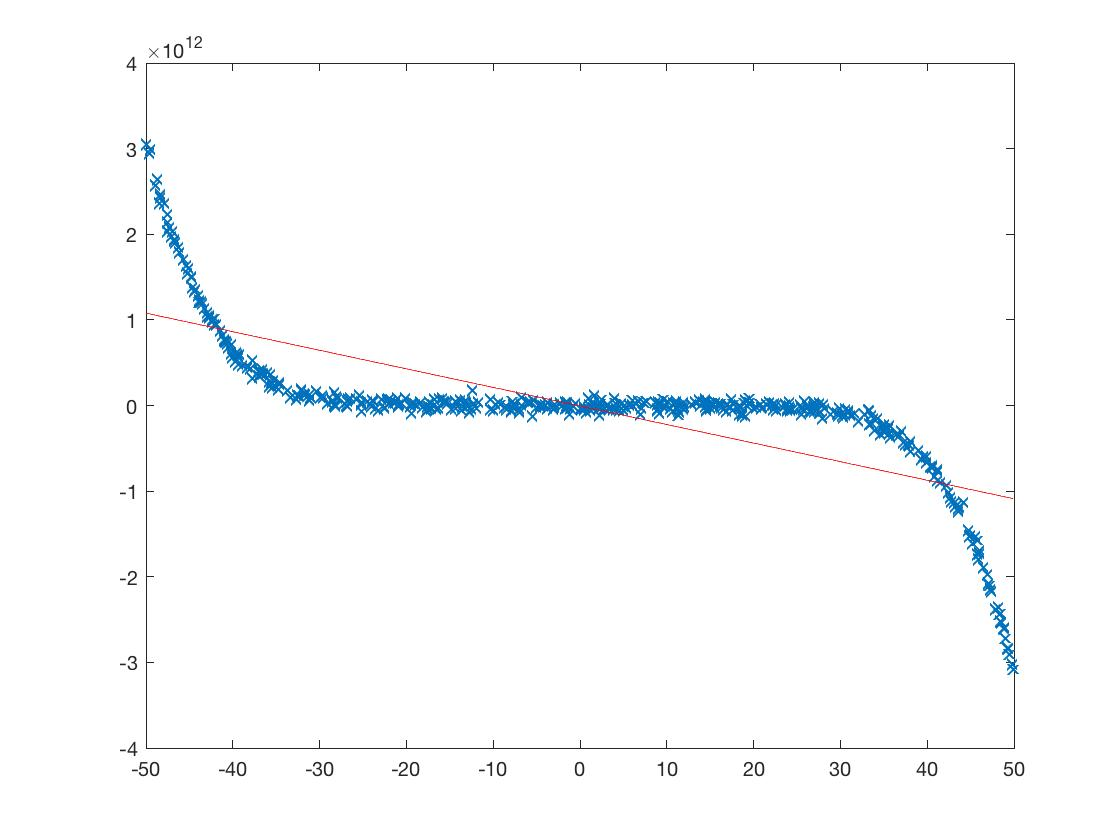
\includegraphics[width = .45\textwidth]{figure/d2.jpg}
}
\\
\centering
\subfigure[d=3]{
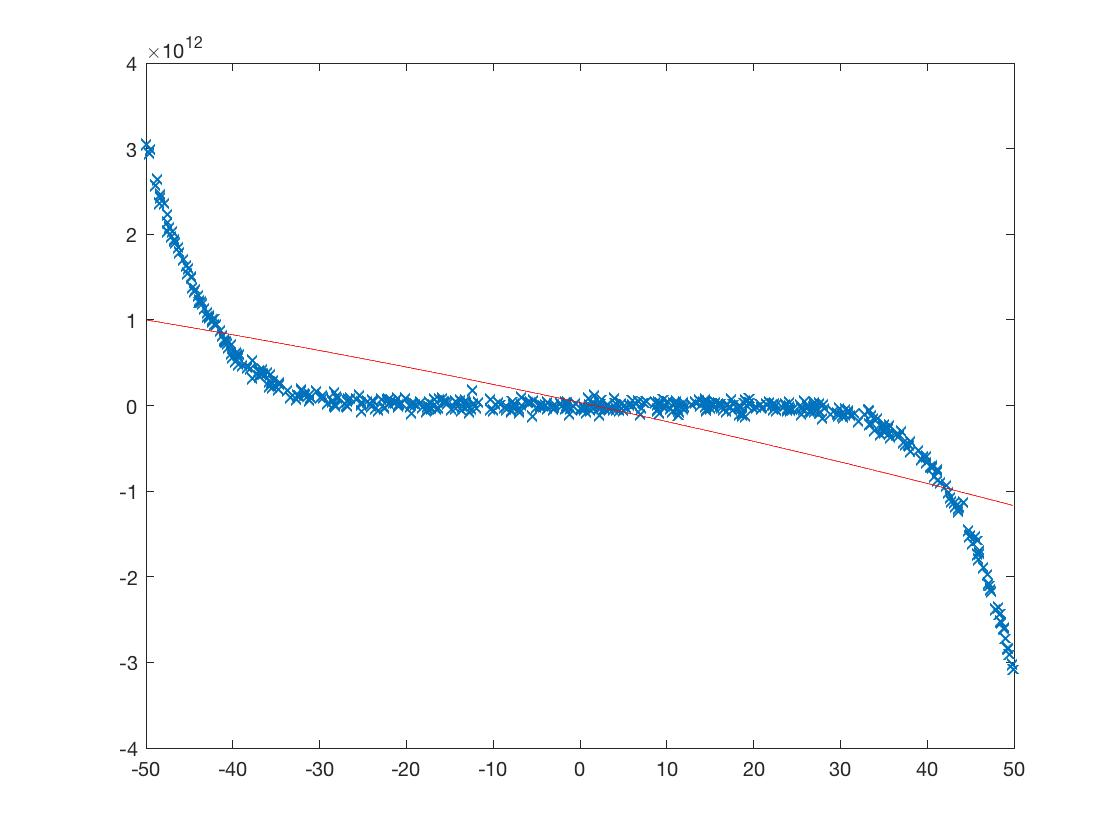
\includegraphics[width = .45\textwidth]{figure/d3.jpg}
}
\subfigure[d=5]{
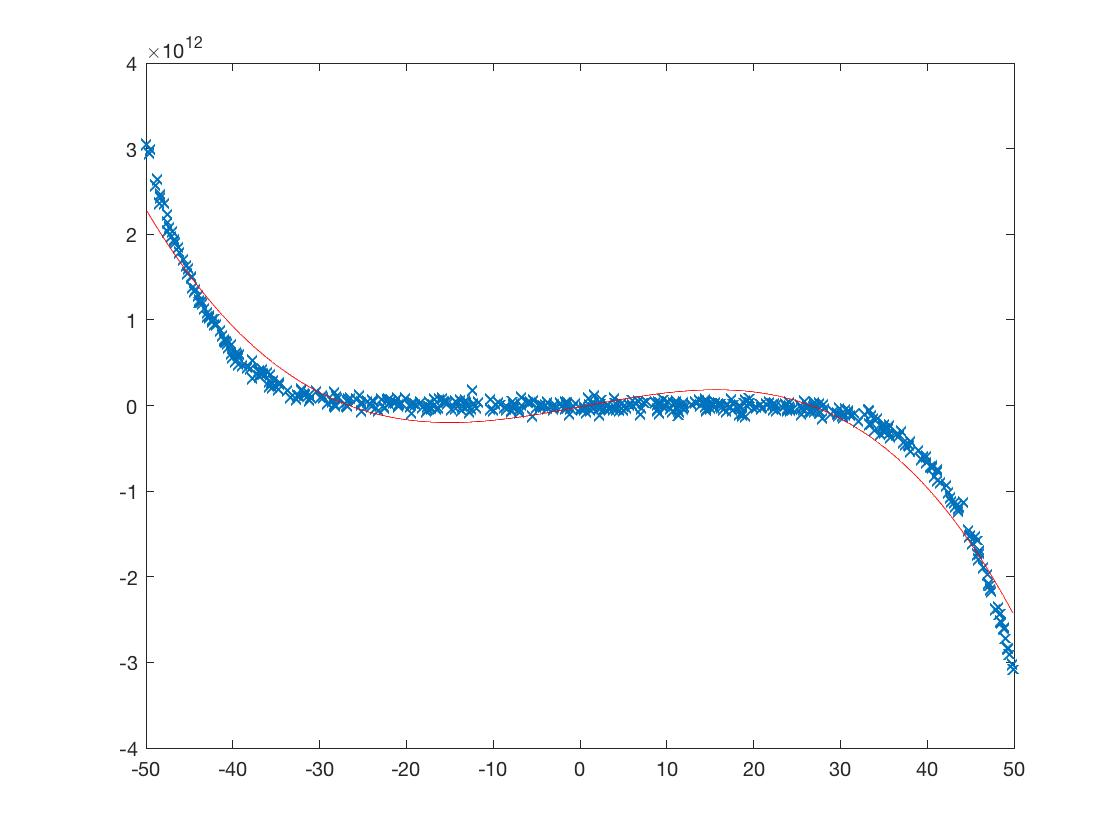
\includegraphics[width = .45\textwidth]{figure/d5.jpg}
}
\end{figure}
\\
\begin{figure}[h]
\centering
\subfigure[d=10]{
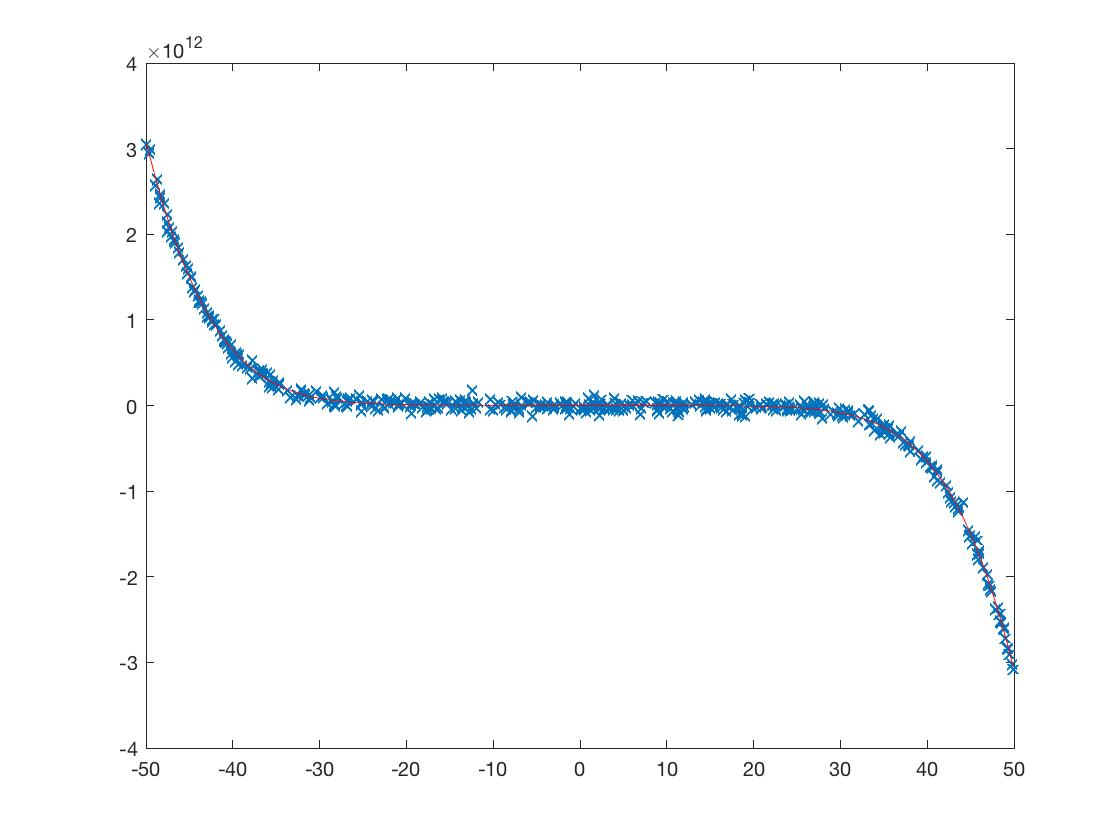
\includegraphics[width = .45\textwidth]{figure/d10.jpg}
\label{Fig.sub.1}
}
\subfigure[d=20]{
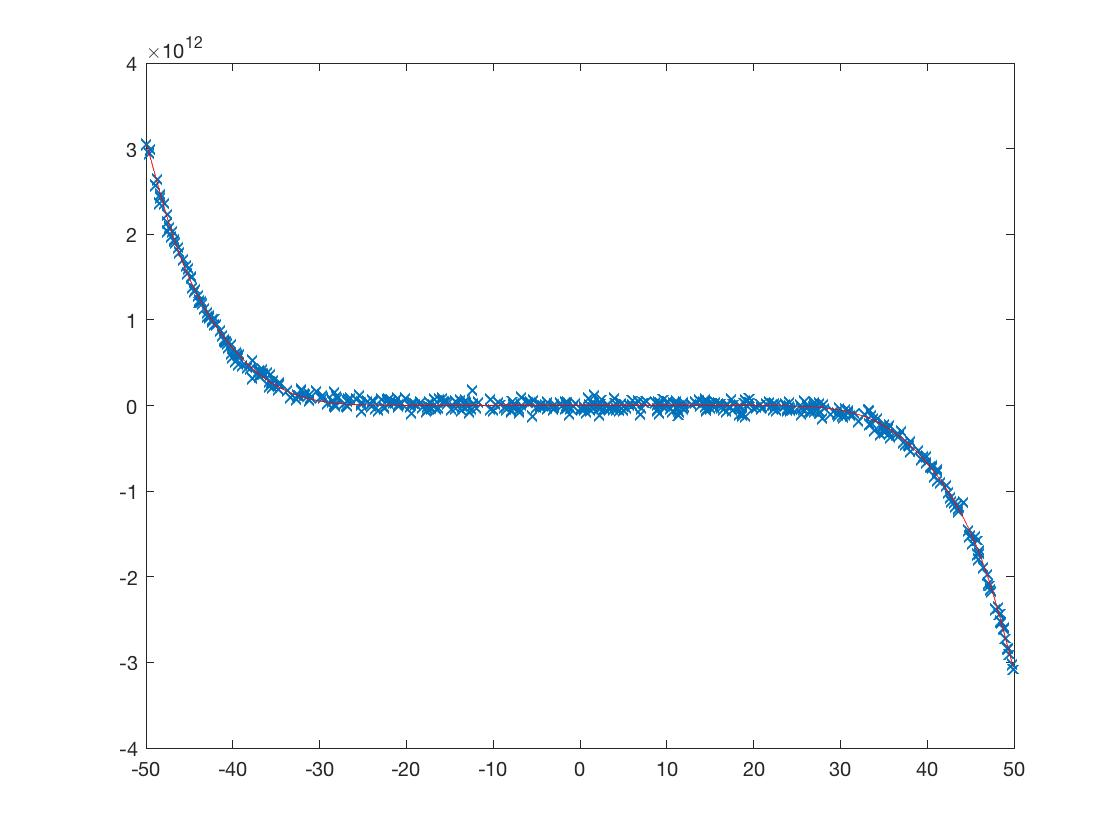
\includegraphics[width = .45\textwidth]{figure/d20.jpg}
\label{Fig.sub.2}
}
\end{figure}
\\
\begin{figure}[h]
\centering
\subfigure[d=30]{
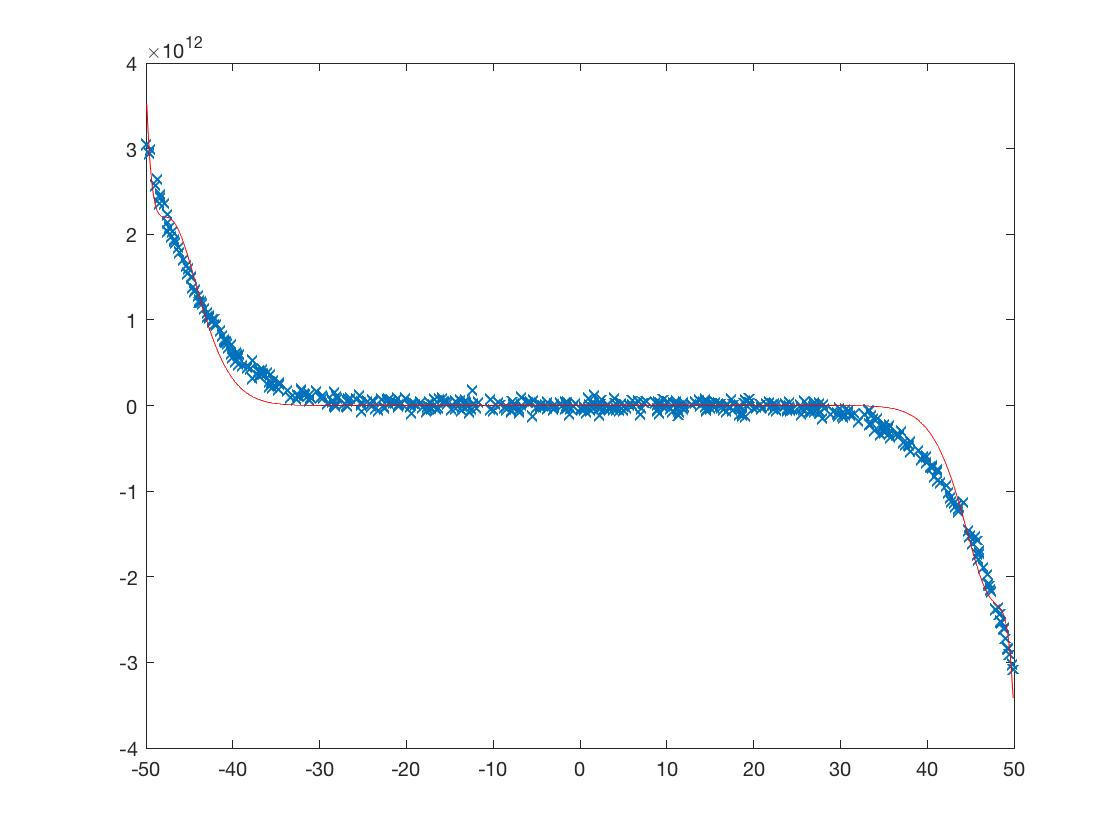
\includegraphics[width = .45\textwidth]{figure/d30.jpg}
}
\subfigure[d=40]{
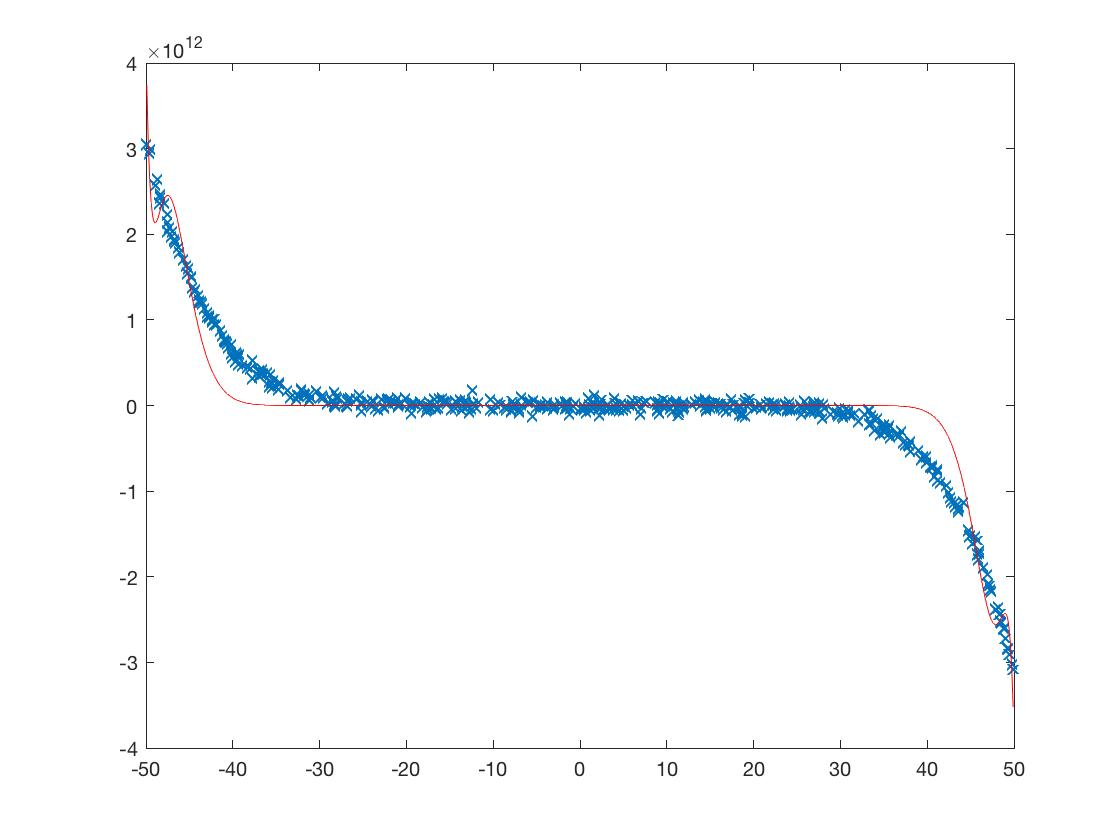
\includegraphics[width = .45\textwidth]{figure/d40.jpg}
}
\end{figure}
\\
Obviously the functions from \ref{Fig.sub.1} and \ref{Fig.sub.2} best fit the data set.Through cross-validation, we can get the best d 11, which is corresponded to the lowest loss on testing set,  as shown in \ref{loss-p-p1} and \ref{overlaid_p1}:
\\
\begin{figure}[h]
\centering
\subfigure[loss-d]{
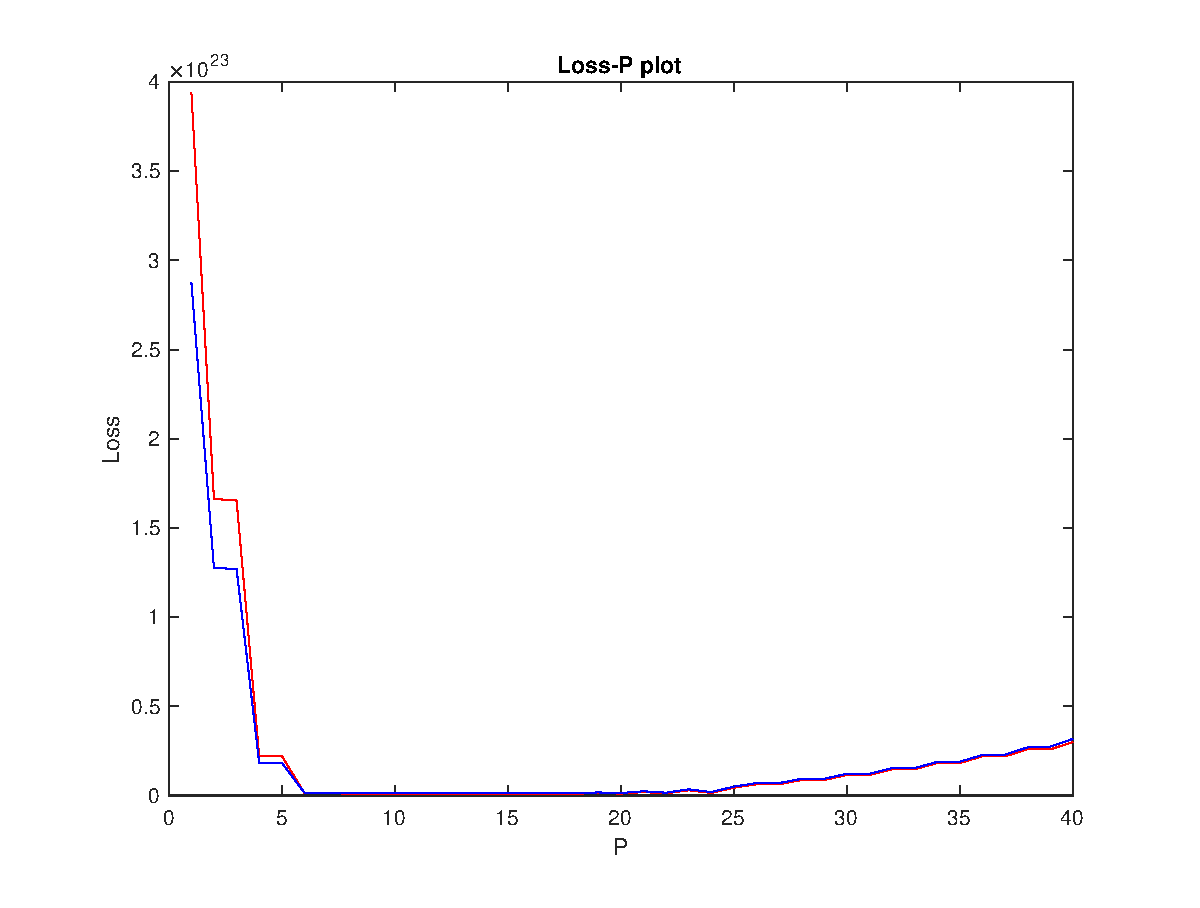
\includegraphics[width= .45\textwidth]{figure/loss-p_p1.eps}
\label{loss-p-p1}}
\subfigure[overlaid]{
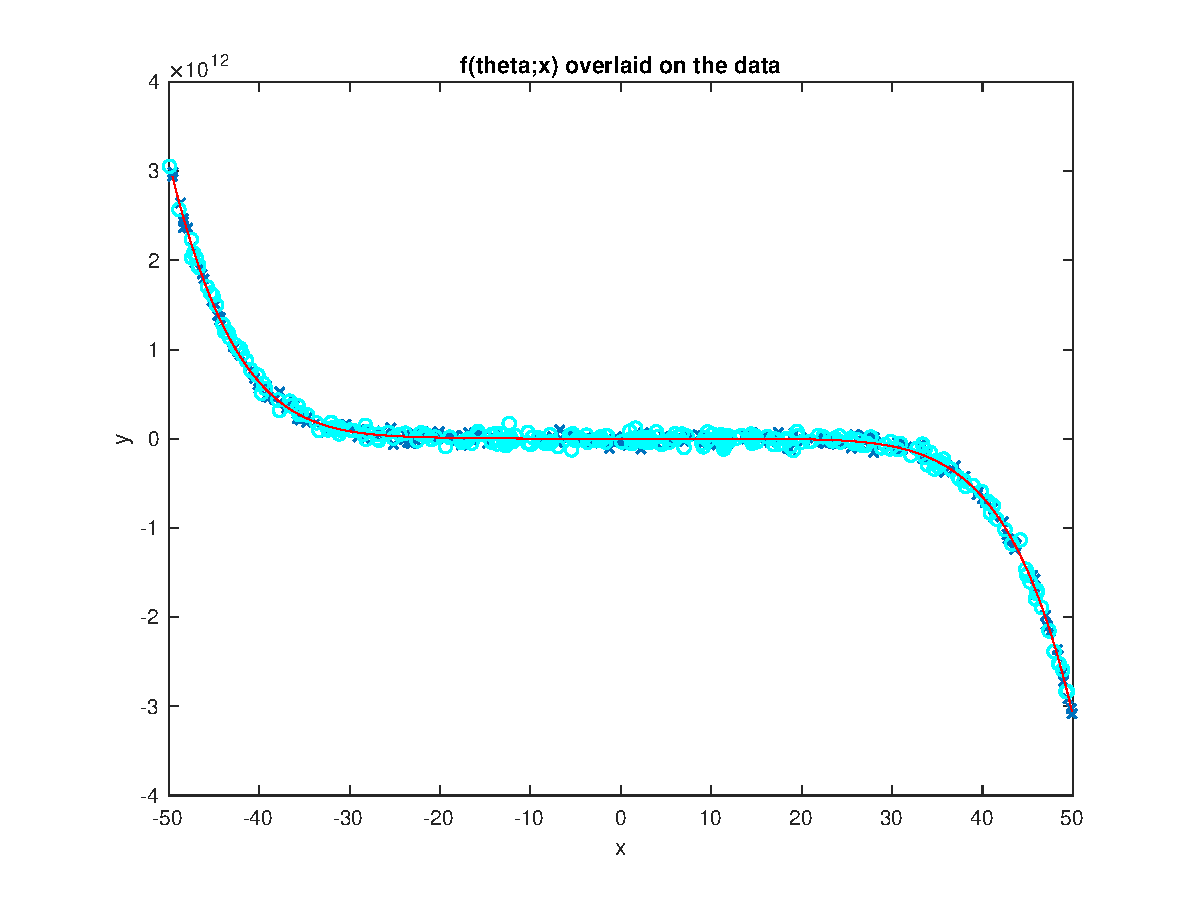
\includegraphics[width= .45\textwidth]{figure/overlaid_p1.eps}
\label{overlaid_p1}
}
\end{figure}
\\

\section{Problem 2}

Use regularized risk minimization to get models, and select the best $\lambda=804$ corresponded to the lowest testing loss, which is shown in $\ref{regr1}$ and $\ref{regr2}$

\begin{figure}[h]
\setcounter{subfigure}{10}
\centering
\subfigure[$\lambda$]{
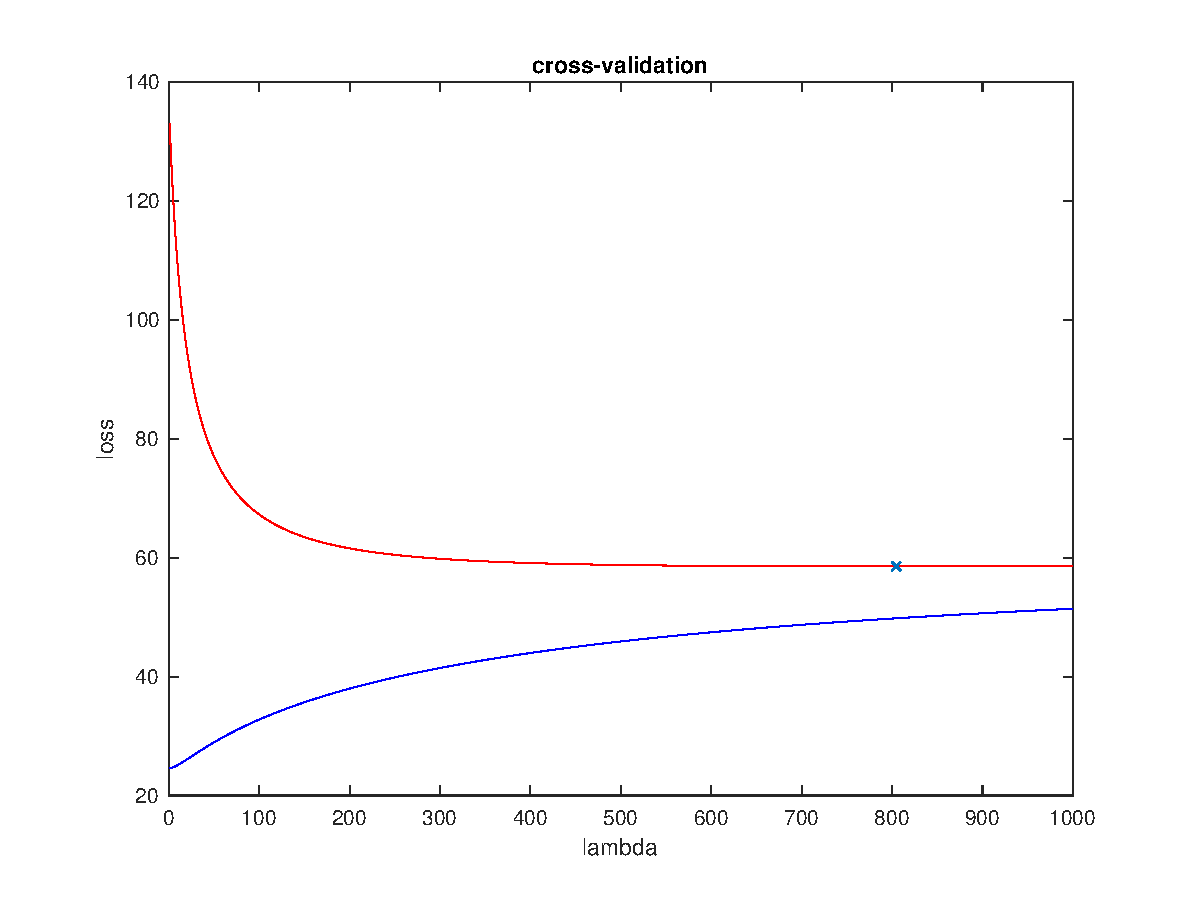
\includegraphics[width = .45\textwidth]{figure/regularization.eps}
\label{regr1}
}
\subfigure[$\frac{1}{\lambda}$]{
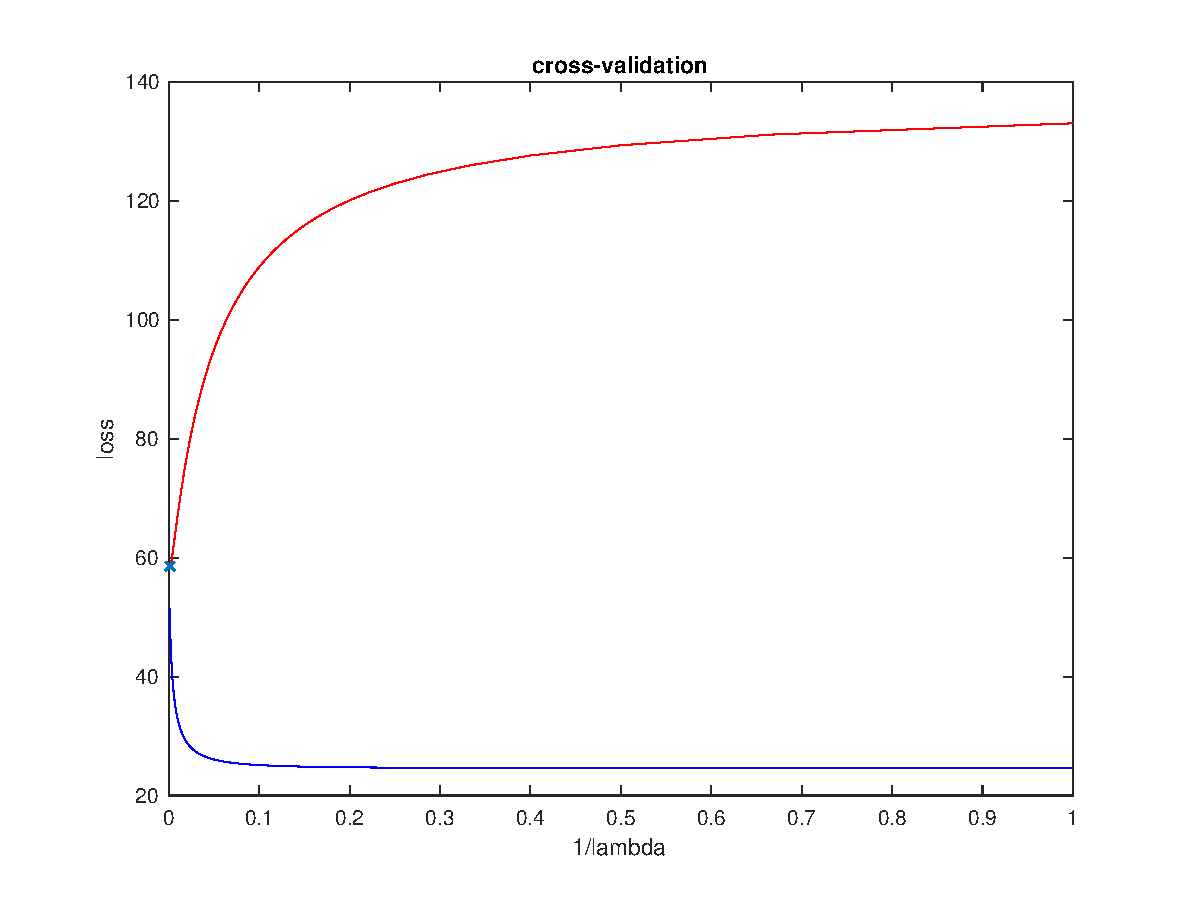
\includegraphics[width = .45\textwidth]{figure/regularizationlambda.eps}
\label{regr2}
}
\end{figure}

\section{Problem 3}
\subsection{}
Proof:
\begin{align}
g(-z) & = \dfrac{1}{1+e^z}  \nonumber\\
       & = \dfrac{e^{-z}}{1+e^{-z}} \nonumber \\
       &= 1 - \dfrac{1}{1+e^{-z}} \nonumber\\
       &= 1 - g(z)  \nonumber
\end{align}

\subsection{}
Proof: suppose: y = g(z) \\ 
\begin{align}
g^{-1}(y)  & = \ln{\dfrac{y}{1-y}} \nonumber \\
               & = \ln{y} - \ln{(1-y)} \nonumber\\ 
               & = \ln{g(z)} - \ln{(1-g(z))} \nonumber\\
               &  = \ln{(\dfrac{1}{1+e^{-z}})} - \ln{(\dfrac{e^{-z}}{1+e^{-z}})} \nonumber\\ 
               & = 0 - \ln{(1-e^{-z})} + \ln{(1+e^{-z})} + \ln{e^{-z}} \nonumber\\ 
               & = z  \nonumber
\end{align}
Therefore,  its inverse is given by $g^{-1}(y) = \ln{(y/(1- y))}$.


\section{Problem 4}
For the function: 
\begin{align}
f(\textbf{x};\theta) = (1+\exp(-\theta^{\mathsf{T}}\textbf{x}))^{-1} \nonumber
\end{align}
with the loss function:
\begin{align}
L = (1-y_i)\log(1-f(x_i, \theta)) - y_i \log(f(x_i, \theta)) \nonumber
\end{align}

We were supposed to solve the gradient descent with derivation: $\nabla_{\theta}R = 0$

\begin{align}
\nabla_{\theta}R &= \frac{1}{N} \sum^{N}_{i=1} \left[\frac{(1-y_i)}{1-f(x_i; \theta)} - \frac{y_i}{f(x_i; \theta)} \right] f^{'}(x_i;\theta) \nonumber\\
& = \frac{1}{N} \sum^{N}_{i=1} \left[ \frac{(1-y_i)(1+e^{-\theta^{\mathsf{T}}x_i})}{e^{-\theta^{\mathsf{T}}x_i}}  - y_i(1+e^{-\theta^{\mathsf{T}}x_i}) \right] \frac{x_i e^{-\theta^{\mathsf{T}}x_i}}{(1+e^{-\theta^{\mathsf{T}}x_i})^2} \nonumber\\
& = \frac{1}{N} \sum^{N}_{i=1} \left[ \frac{(1-y_i)x_i}{1+e^{-\theta^{\mathsf{T}}x_i}} - \frac{y_i x_i e^{-\theta^{\mathsf{T}}x_i}}{1+e^{-\theta^{\mathsf{T}}x_i}}  \right] \nonumber \\
& = \frac{1}{N} \sum^{N}_{i=1} \left[  (1-y_i)x_i - y_i x_i e^{-\theta^{\mathsf{T}}x_i}\right] (1+e^{-\theta^{\mathsf{T}}x_i})^{-1}   \nonumber
\end{align}

However, this equation is too complicated to solve analytically, with some numerical method we can let the results of parameters approach to the best model. 

Set the iteration to be 100000, with tolerance $\epsilon = 0.001$ and steps $\ita = 1$, the 2D X binary boundary given by $ \theta_1 \times x_1 + \theta_2 \times x_2  + \theta_3 = 0$ and the classification error and empirical risk obtained from the process are shown as $\ref{41(2)}$ and $\ref{41(1)}$.

The model obtained is $\theta = [48.8850, 26.8971, -19.2476]$.

\begin{figure}[h]
\setcounter{subfigure}{12}
\centering
\subfigure[binary boundary 1]{
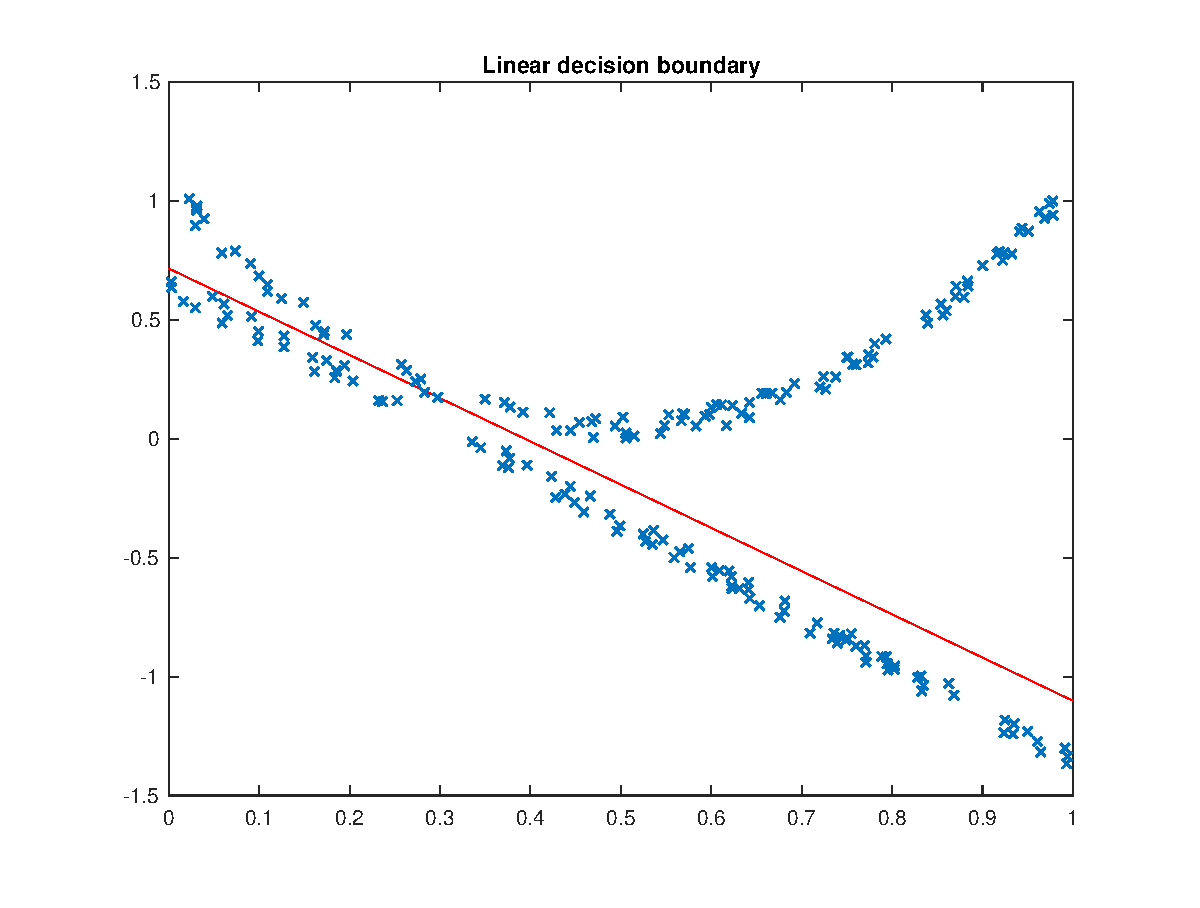
\includegraphics[width = .45\textwidth]{figure/4_1(2).eps}
\label{41(2)}
}
\subfigure[error and risk 1]{
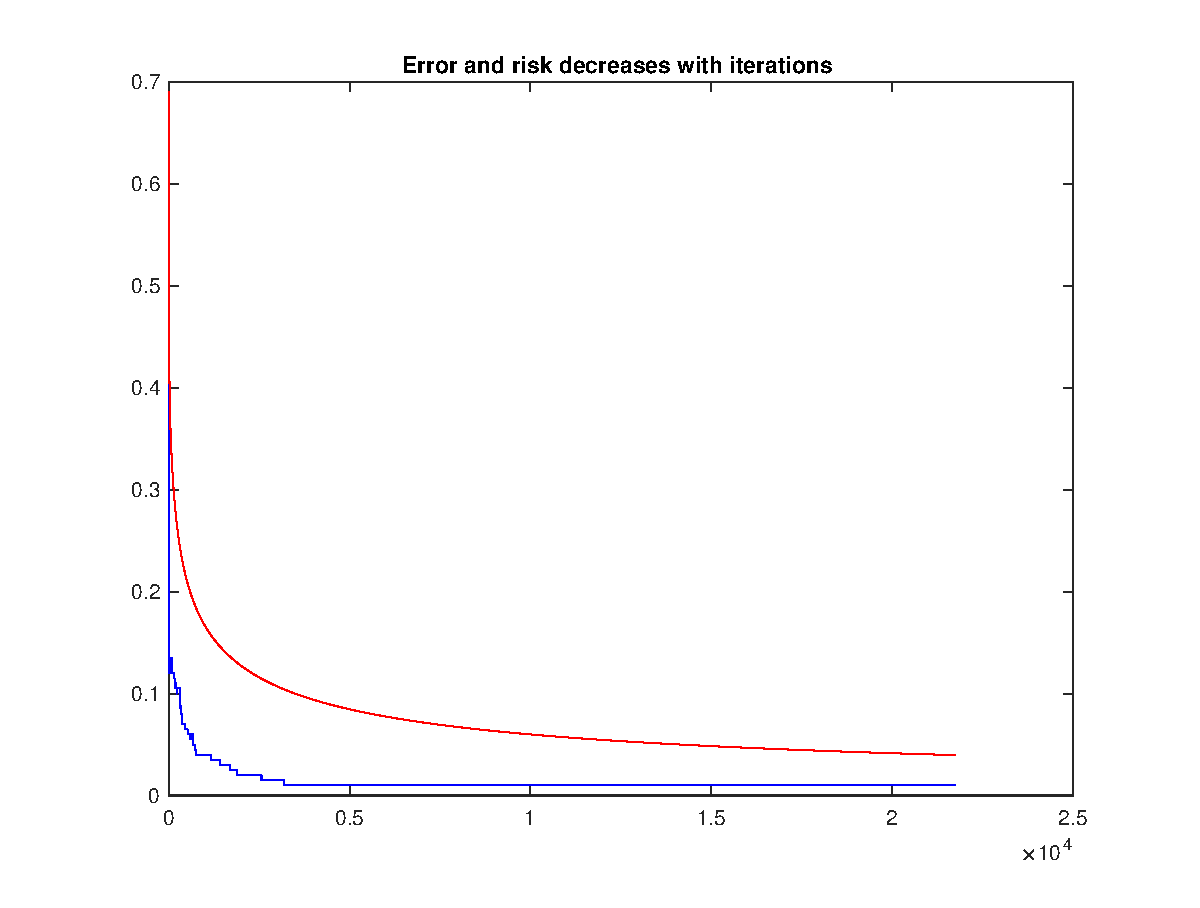
\includegraphics[width = .45\textwidth]{figure/4_1(1).eps}
\label{41(1)}
}
\end{figure}

Set the iteration to be 200000, with tolerance $\epsilon = 0.001$ and steps $\ita = 2$, the model will be as shown as $\ref{42(2)}$ and $\ref{42(1)}$.

The model obtained is $\theta = [ 68.6228, 36.5855, -26.4124]$.

\begin{figure}[h]
\setcounter{subfigure}{14}
\centering
\subfigure[binary boundary 2]{
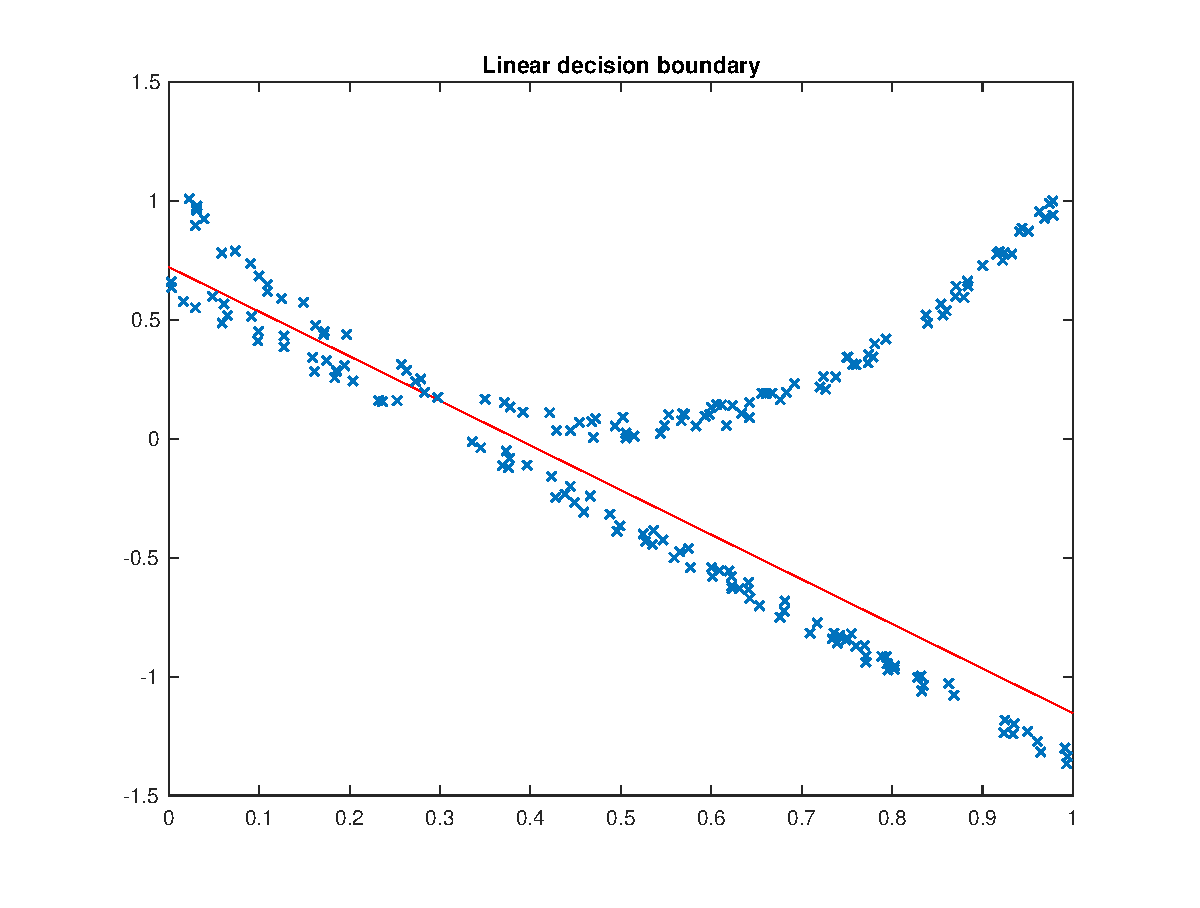
\includegraphics[width = .45\textwidth]{figure/4_2(2).eps}
\label{42(2)}
}
\subfigure[error and risk 2]{
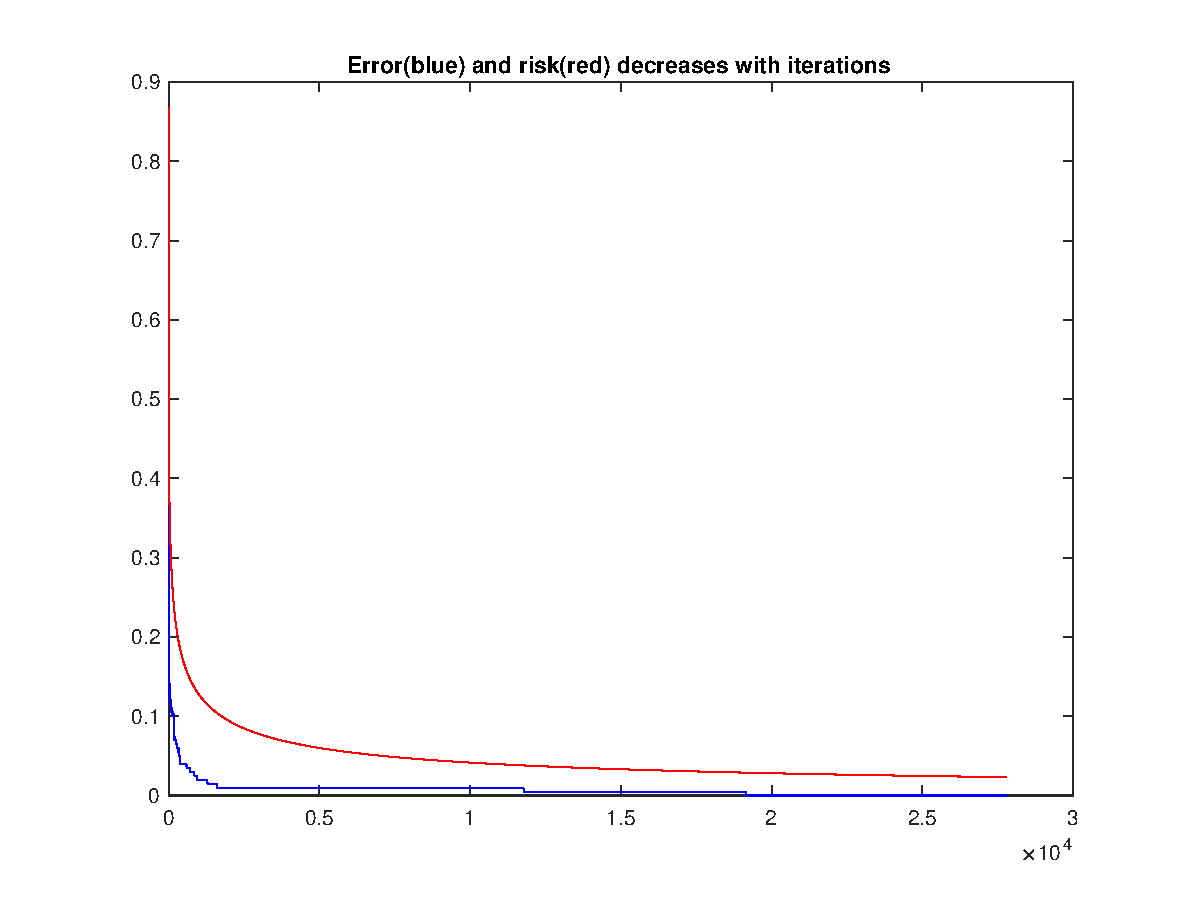
\includegraphics[width = .45\textwidth]{figure/4_2(1).eps}
\label{42(1)}
}
\end{figure}

Set the iteration to be 500000, with tolerance $\epsilon = 0.001$ and steps $\ita = 1$, the model will be as shown as $\ref{43(2)}$ and $\ref{43(1)}$.

The model obtained is $\theta = [48.8852, 26.8971, -19.2477]$, so the iteration doesn't affect the final results as it's the same as the first case.

\begin{figure}[h]
\setcounter{subfigure}{16}
\centering
\subfigure[binary boundary 3]{
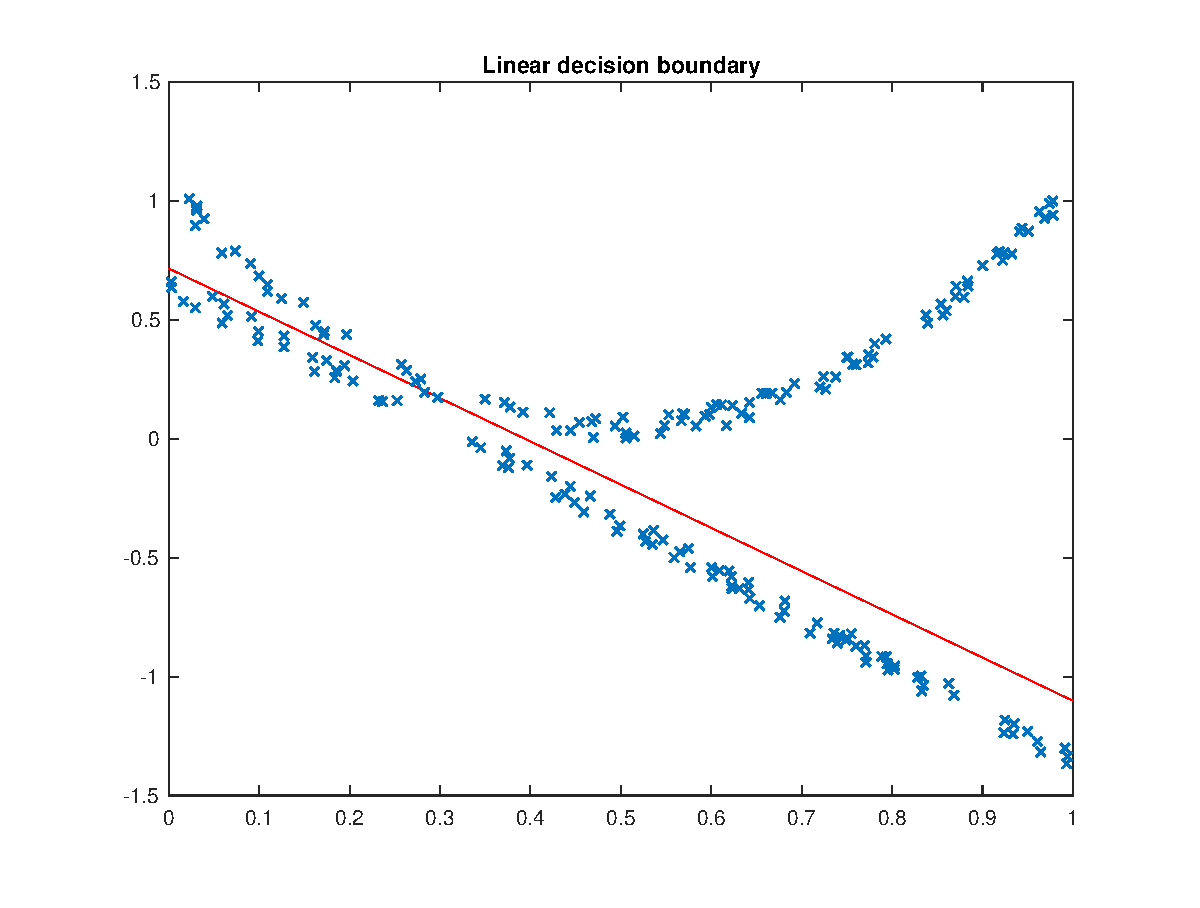
\includegraphics[width = .45\textwidth]{figure/4_3(2).eps}
\label{43(2)}
}
\subfigure[error and risk 3]{
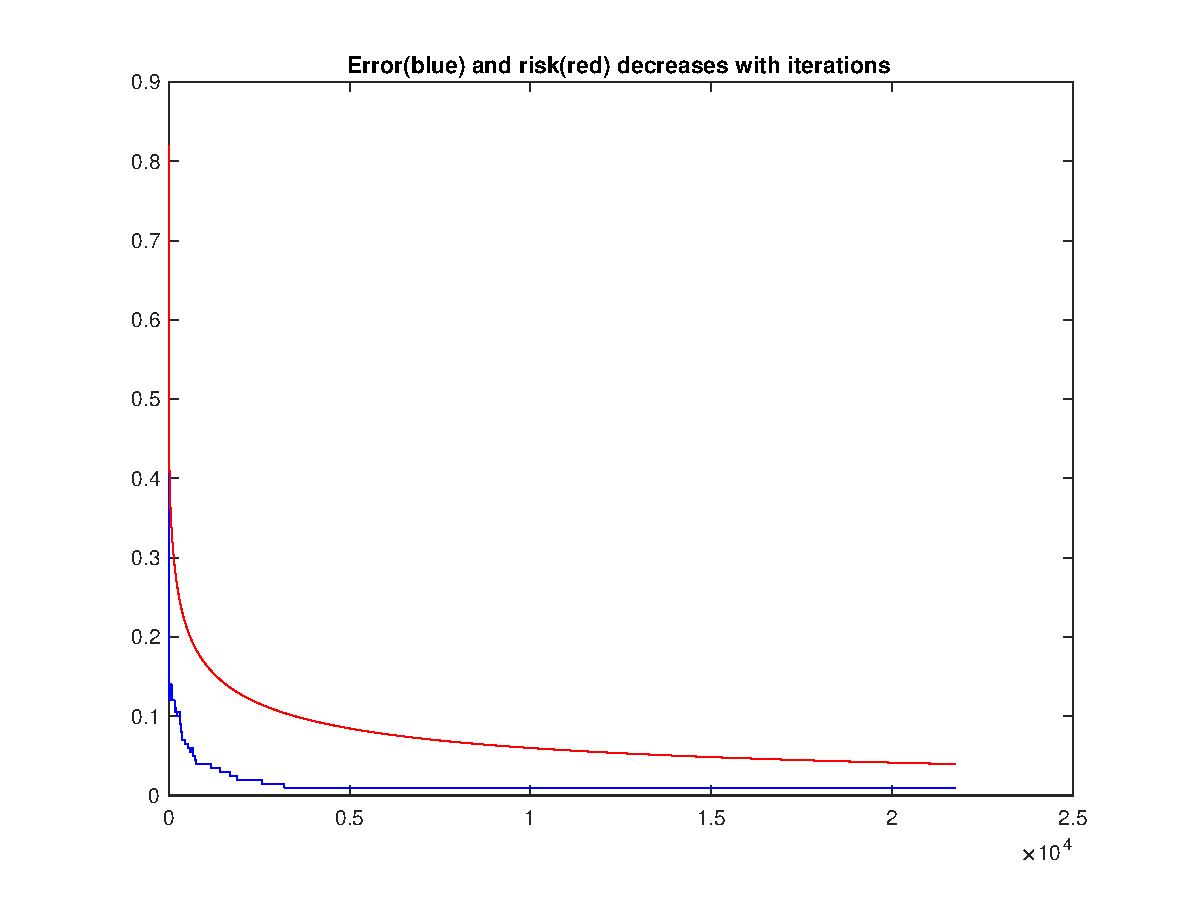
\includegraphics[width = .45\textwidth]{figure/4_3(1).eps}
\label{43(1)}
}
\end{figure}

Since the whole data set is used for training, the model may be overfitting when the conditions change.

\section{annotion}

The matlab source file \textit{polyregcv.m} is for problem 1, it calls the function \textsl{polyreg()} provided by \textit{polyreg.m} which is downloaded from the website, the \textit{multivariable.m} and \textit{regrimin.m} are for problem 2, and the \textit{LRGD.m} is for problem 4.

\end{document}